\documentclass{report}
 \usepackage{lipsum}
 \usepackage[margin=1in,left=1.5in,includefoot]{geometry}
\usepackage{graphicx} %allows you to get photos 
\usepackage{float} 
\usepackage{blindtext}
\usepackage[utf8]{inputenc}
\usepackage{wrapfig,lipsum}
\usepackage{parallel,enumitem}
\usepackage{hyperref}
\usepackage{listings}
\usepackage[table]{xcolor}
\usepackage[T1]{fontenc}
\usepackage{inconsolata}

\usepackage{color}

\definecolor{pblue}{rgb}{0.13,0.13,1}
\definecolor{pgreen}{rgb}{0,0.5,0}
\definecolor{pred}{rgb}{0.9,0,0}
\definecolor{pgrey}{rgb}{0.46,0.45,0.48}

\usepackage{listings}
\lstset{language=Java,
  showspaces=false,
  showtabs=false,
  breaklines=true,
  showstringspaces=false,
  breakatwhitespace=true,
  commentstyle=\color{pgreen},
  keywordstyle=\color{pblue},
  stringstyle=\color{pred},
  basicstyle=\ttfamily,
  moredelim=[il][\textcolor{pgrey}]{$$},
  moredelim=[is][\textcolor{pgrey}]{\%\%}{\%\%}
}

\begin{document}


\begin{titlepage}
	\centering
	{\scshape\LARGE  \par}
	\vspace{1cm}
	{\scshape\Large Graph Models and Simulation Research  \par}
	\vspace{1.5cm}
	{\huge\bfseries Overview Mavlink and MSP Protocols \par}
	\vspace{1cm}
	{\huge\itshape Hesham Hosney\par}
        \vspace{2cm} 
	{\Large Supervisor:\par } 
	{\huge Prof. Dr. Umut Durak\par}
\vspace{.5cm} 

\vfill
% Bottom of the page
	{\large \today\par}
\end{titlepage}


\cleardoublepage
\tableofcontents
\listoffigures
\cleardoublepage



\begin{abstract}


In this report, we briefly describe Mavlink and MSP protocols our main aim is to provide structured documentation, which maps the relation between Mavlink and MSP common messages. we will start with an introductory chapter discussing the main flight stack and commonly used technology, an overview of Mavlink Protocol, and Multiwii Serial protocol.
chapter 2 we will focus on our main goal which is mapping the messages between the two protocols.
We conclude our findings the conculsion chapter.


\end{abstract}
%\cleardoublepage
%\centerline{\bfseries Statement of Originality}
%	\vspace*{1em}
%	\noindent
%	This research project has been performed independently with the support of my supervisors.
%	To the best of the author's knowledge, this research project contains no material previously
%	published or written by another person except where due reference is made in the text.
%
%\cleardoublepage

\chapter{Introduction}

Drone Software developments are gaining business and commercial interests.
The industry is set to become the next high growth market with very high potential and exponential growth.

\section{System Overview}


In high-level abstraction, the components of the flight stack consist of three main components ground control station, drone, and Communication Layer.
\hyperref[fig:systemoverview]{Figure 1.1} Describes the system overview. 
 \begin{figure}[H]
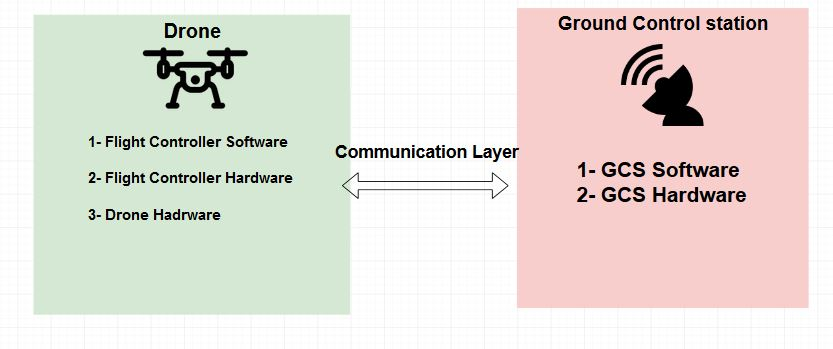
\includegraphics[width=12cm,height=10cm]{images/1.jpg}
\caption{Flight Stack Overview}
\label{fig:systemoverview}
\end{figure}
\cleardoublepage



\noindent \textbf{The Ground Control Station} is mainly an offboard computer that can communicate with the drone to gather information, for instance, location speed battery info. in addition, it's also can send a command to do certain behaviors like landing the drone or directing the drone to a specific destination.
It could also preceived as a computer with USB in a telemetry module there is also software or a user interface layer for doing specific functionality and sending commands using Mavlink communication protocol. for example Dronekit, which is a software for controlling the drone using Python. 

\textbf{Drone Hardware} consists of motors GPs probes that made up the drone.
The Flight Control Hardware is connected to Drone Hardware like Navio2 based on Rasperrypi
The flight controller software is a compiled code that uploaded to the autopilot hardware that controls the drone's basic components For example, the open source px4 and ardupilot. Additionally, the Drone hardware and the flight controller hardware could be replaced by Software in the Loop SITL it's mainly a simulation running on the computer that facilitates the whole process as a virtual instance this will practice and facilitate testing. \\ 

\textbf{Communication Layer} is a standard protocol that used for the communication between the ground control station and the drone in a bidirectional way, in another word it is like a standard collection of messages. Mavlink[1] has a standard message structure each Mavlink message has the same message structure allowing the sending node to package the information in a consistent manner and the receiving node to interpret the incoming data consistently. Every message has a message ID which a number that has an objective meaning. for example, a heartbeat is a message with id 0 when which means the drone is active.



\section{Mavlink Message Structure}


Each Mavlink message consists of 6 bytes for the header and 9 bytes for the payload and 2 bytes for the checksum for verifying the message integrity and assuring that the message wasn’t altered during the transmission. The header contains a packet start sign encoded into one byte which indicates the starting of the packet.
\begin{itemize}
  \item Each message starts with 0xFE indicates the starting of a new message.
  \item Payload length indicates the length of the following payload.
  \item Packet sequence for sequencing the packets thus it’s a method to detect packet loss.
\item System Id to identify the system ground always 1-255 similar to IP address 1 for the drone and 255 for the ground control station.
\item Component id to identify the component sending the message inside the system usually zero it’s similar to the port number but not widely used.
\item Message-id: identify the type of message in the payload for instance 0 is the heartbeat 33 it means the message is carrying out the GPs coordinates.
\item Data: payload and it depends on the message-id.
\item Last two bytes are for identifying the checksum.
\end{itemize}

\hyperref[fig:Mavlinkmessage]{Figure 1.2} Describes Mavlink message structure. 
 \begin{figure}[H]
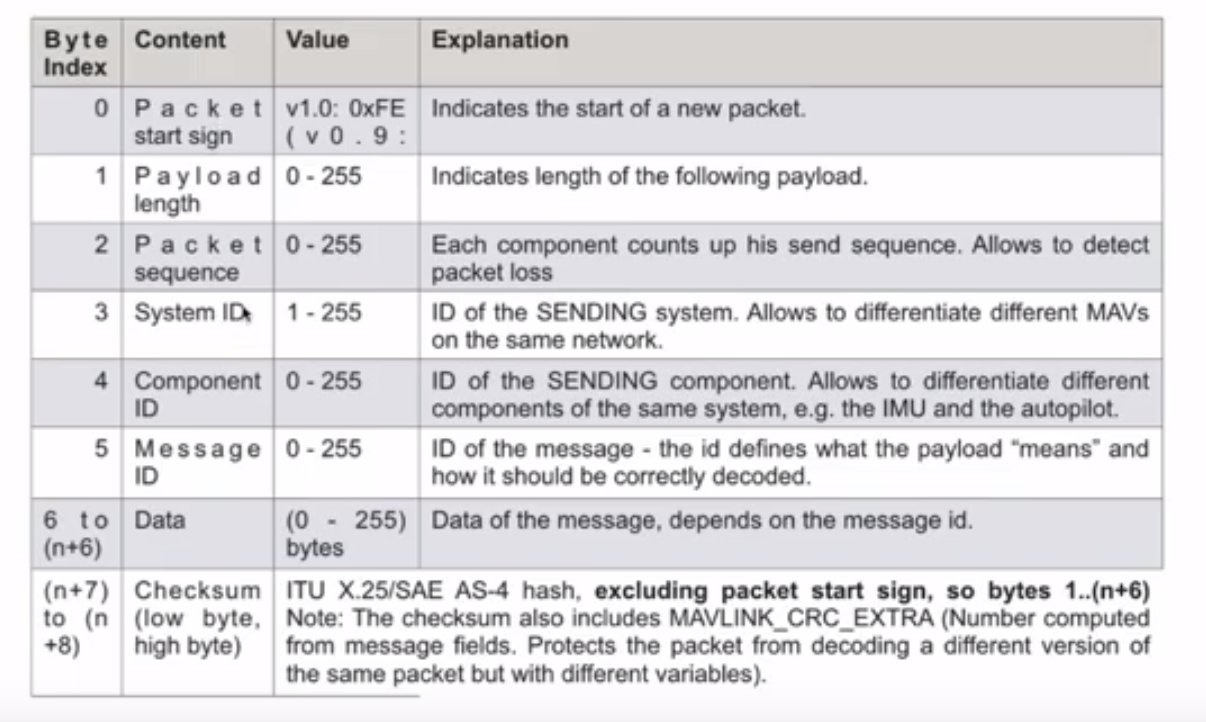
\includegraphics[width=15cm,height=10cm]{images/2.png}
\caption{Mavlink Message Structure }
\label{fig:Mavlinkmessage}
\end{figure}

\cleardoublepage



\section{Multiwii Serial Protocol MSP}

MSP MultiWii Serial Protocol[2] is the de-facto standard to interact with a MultiWii flight controller (FC). Its implementation contains a list of the most common operations one would expect from a remote control/telemetry point of view. Developers can add custom functionality if required,
They are three type of messages in MSP protocol. 
\begin{itemize}
  \item  command – is an incoming (into FC) message without implicit outgoing response from the controller
  \item  request –  is an incoming message with implicit outgoing response (e.g. a telemetry request sent in by a remote station)
  \item  response – is the outgoing message resulting from an incoming request. 
\end{itemize}

\subsection{Header}
The header is three bytes and contains the message start characters \$M and a character showing which direction the message is going. <  denotes going to the flight controller (command and request), > denotes coming from the flight controller (response).

\subsection{Size}
The fourth byte is the length (in bytes) of the data section. For example, if the data section had three INT 16 variables then the size byte would be 6.

\subsection{Type}
The 5th byte is the type of MSP message similar to Mavlink message ID. Value 1xx identify requests while 2xx identify commands.
A full list of MSP[2]

\subsection{Data}
The data is where all the information is sent. Request messages have no data in them. Commands and responses do, because they contain information.

\subsection{Checksum}
The final byte of an MSP message is the checksum. "The checksum is the XOR of size, type and payload bytes". For a request message the checksum is equal to the type.

\hyperref[fig:msp]{Figure 1.3} Depicts MSP message structure. 
 \begin{figure}[H]
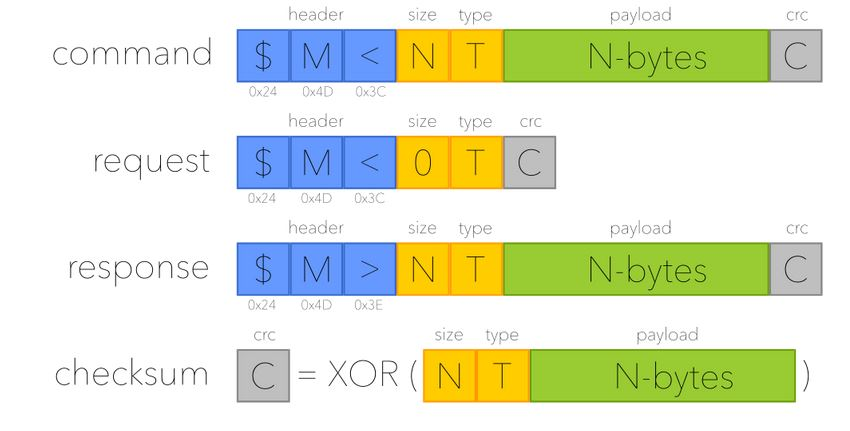
\includegraphics[width=15cm,height=10cm]{images/3.jpg}
\caption{MSP Message Structure }
\label{fig:msp}
\end{figure}




\chapter{Messages Reference}
\section{Introduction} 
In this chapter, we document all Mavlink messages, which have a corresponding MSP message.
As a noticed there are way more MAvlink messages that have no corresponding MSP message.
We mapped messages on the table as Following.
\begin{itemize}
  \item For every Mavlink message, we started with the message name and number and description.
  \item We wrote Mavlink message field name and type in a comma-separated for instance system\_status,u8 this means the field part of the message is system\_status and the data type representing it is unsigned int 8 bits.
  \item  We mapped the corresponding MSP message which does the same functionality with the message name,Message-ID, Field name(data), and Field type.   
\end{itemize}


\subsection{Compatibility  Matrix \\} 
Messages were highlighted with the following colors as an indication of the compatibility between Mavlink and MSP
\begin{itemize}
  \item Green: this means the messages on both protocol are fully compatibile.    
  \item Light Grey: This means they are partially compatible however there are differences in both protocols, for instance, the data type in one protocol is int with 8 bits and unsigned int on the other.
  \item Yellow: This means there is no compatibility between the messages for example we didn't find an MSP message that corresponds to this particular message on Mavlink. 
\end{itemize}
\cleardoublepage

\section{Messages Reference}

\subsection{HeartBeat 0} 

The heartbeat message shows that a system or component is present and responding. The type and autopilot fields (along with the message component id), allow the receiving system to treat further messages from this system appropriately (e.g. by laying out the user interface based on the autopilot).  \\

{\rowcolors{2}{green!80!yellow!50}{green!80!yellow!50}
\centering
\begin{tabular}{ |p{4cm} |p{7cm} | p{2cm}|m{5em}|}
\hline
Mavlink Message Field(Name,type)&Corresponding MSP Message(Name,id,data,type)& Compatibility & Notes\\
\hline
type,u8 & MSP\_IDENT,100,MULTITYPE,u8  & Yes & - \\
\hline
\rowcolor{yellow}
autopilot & Not Found & No& -\\
\hline
\rowcolor{yellow}
base\_mode,u8 & No Found & No  & -  \\
\hline
\rowcolor{yellow}
custom\_mode,u32& Not Found & No & - \\
\hline
\rowcolor{yellow}
system\_status,u8 & Not Found & No & - \\
\hline
mavlink\_version,u8& MSP\_IDENT,100,MSP\_VERSION,u8  & Yes & - \\
\end{tabular}
}
\cleardoublepage


\subsection{SYS\_STATUS 1} 
The general system state. If the system is following the MAVLink standard, the system state is mainly defined by three orthogonal states/modes: The system mode, which is either LOCKED (motors shut down and locked), MANUAL (system under RC control), GUIDED (system with autonomous position control, position setpoint controlled manually) or AUTO (system guided by path/waypoint planner). The NAV\_MODE defined the current flight state: LIFTOFF (often an open-loop maneuver), LANDING, WAYPOINTS or VECTOR. This represents the internal navigation state machine. The system status shows whether the system is currently active or not and if an emergency occurred. During the CRITICAL and EMERGENCY states the MAV is still considered to be active, but should start emergency procedures autonomously. After a failure occurred it should first move from active to critical to allow manual intervention and then move to emergency after a certain timeout. \\

{\rowcolors{2}{yellow}{yellow}
\centering
\begin{tabular}{ |p{5cm} |p{7cm} | p{2cm}|m{5em}|}
\hline
Mavlink Message Field(Name,type)&Corresponding MSP Message(Name,id,data,type)& Compatibility & Notes\\
\hline
onboard\_control\_sensors\_present,u32 & Not Found & No & - \\
\hline
\hline
onboard\_control\_sensors\_enabled,u32 & Not Found & No & - \\
\hline
onboard\_control\_sensors\_health,u32 & Not Found & No & - \\
\hline
load,u16 & Not Found & No & - \\
\hline
\rowcolor{lightgray}
voltage\_battery,u16 & MSP\_ANALOG,110,vbat,u8 & Partially &  Mavlink u16 ,unit is mv MSP u8, unit 0.1 volt  \\
\rowcolor{lightgray}
\hline
current\_battery,i16 &  MSP\_ANALOG,110,amperage,u16 & Partially & Mavlink i16 MSP u16 \\
\hline
\rowcolor{lightgray}
battery\_remaining,i8 & MSP\_MISC,114,conf.vbatscale,u8 & Partially &  Mavlink i8, MSP u8  \\
\hline
drop\_rate\_comm,u16 & Not Found & No & - \\
\hline
\rowcolor{green}
errors\_comm,u16 & MSP\_STATUS,101, i2c\_errors\_count,u16 & Yes &  - \\
\hline
errors\_count1,u16 & Not Found & No & - \\
\hline
errors\_count2,u16 & Not Found & No & - \\
\hline
errors\_count3,u16 & Not Found & No & - \\
\hline
errors\_count4,u16 & Not Found & No & - \\

\end{tabular}
}
\cleardoublepage



\subsection{GPS\_RAW\_INT 24} 
The global position, as returned by the Global Positioning System (GPS). This is NOT the global position estimate of the system, but rather a RAW sensor value. See message GLOBAL\_POSITION for the global position estimate. \\ 

{\rowcolors{2}{yellow}{yellow}
\centering
\begin{tabular}{ |p{4cm  } |p{7cm} | p{2cm}|m{5em}|}
\hline
Mavlink Message Field(Name,type)&Corresponding MSP Message(Name,id,data,type)& Compatibility & Notes\\
\hline
time\_usec,u32 & Not Found & No & - \\
\hline
port,u8 & Not Found & No & - \\
\rowcolor{green}
\hline
fix\_type,u8 & GPS\_FIX,106,GPS\_FIX,u8 & Yes  & - \\
\rowcolor{lightgray}
\hline
lat,i32 &  	GPS\_coord[LAT],106,GPS\_FIX,u32 & Partially   & Mavlink i32, MSP u32\\
\rowcolor{lightgray}
\hline
long,i32 &  	GPS\_coord[LON],106,GPS\_FIX,u32 & Partially   & Mavlink i32, MSP u32\\
\rowcolor{lightgray}
\hline
alt,i32 &  	GPS\_altitude,106,GPS\_FIX,u16 & Partially   & Mavlink i32, MSP u16\\
\hline
\rowcolor{green}
eph,u16 & MSP\_GPSSTATISTICS,-,eph,u16 & Yes & - \\
\hline
\rowcolor{green}
epv,u16 & MSP\_GPSSTATISTICS,-,eph,u16 & Yes & - \\
\rowcolor{green}
\hline
vel,u16 & GPS\_altitude,106,GPS\_speed,u16 & Yes   & - \\
\hline
cog,u16 & Not Found & No & - \\
\hline
\rowcolor{green}
satellites\_visible,u8 & MSP\_RAW\_GPS,106,GPS\_numSat,u8& Yes & - \\
\hline
cog,u16 & Not Found & No & - \\
\end{tabular}
}

\cleardoublepage





\subsection{RAW\_IMU 27} 
The RAW IMU readings for a 9DOF sensor, which is identified by the id (default IMU1). This message should always contain the true raw values without any scaling to allow data capture and system debugging. \\

{\rowcolors{2}{yellow}{yellow}
\centering
\begin{tabular}{ |p{4cm  } |p{7cm} | p{2cm}|m{5em}|}
\hline
Mavlink Message Field(Name,type)&Corresponding MSP Message(Name,id,data,type)& Compatibility & Notes\\
\hline
time\_usec,u64 & Not Found & No & - \\
\hline
\rowcolor{green}
xacc,i16 &MSP\_RAW\_IMU,102,accx,i16& Yes & - \\
\hline
\rowcolor{green}
yacc,i16 &MSP\_RAW\_IMU,102,accy,i16& Yes & - \\
\hline
\rowcolor{green}
zacc,i16 &MSP\_RAW\_IMU,102,accz,i16& Yes & - \\
\hline
\rowcolor{green}
xgyro,i16 &MSP\_RAW\_IMU,102,gyrx,i16& Yes & - \\
\hline
\rowcolor{green}
ygyro,i16 &MSP\_RAW\_IMU,102,gyry,i16& Yes & - \\
\hline
\rowcolor{green}
zgyro,i16 &MSP\_RAW\_IMU,102,gyrz,i16& Yes & - \\
\hline
\rowcolor{green}
xmag,i16 &MSP\_RAW\_IMU,102,magx,i16& Yes & - \\
\hline
\rowcolor{green}
ymag,i16 &MSP\_RAW\_IMU,102,magy,i16& Yes & - \\
\hline
\rowcolor{green}
zmag,i16 &MSP\_RAW\_IMU,102,magz,i16& Yes & - \\
\hline
id,u8 & Not Found & No & - \\
\hline
temperature,i16 & Not Found & No & - \\

\end{tabular}
}

\cleardoublepage



\subsection{ATTITUDE 30} 
The attitude in the aeronautical frame (right-handed, Z-down, X-front, Y-right).\\

{\rowcolors{2}{yellow}{yellow}
\centering
\begin{tabular}{ |p{4cm  } |p{7cm} | p{2cm}|m{5em}|}
\hline
Mavlink Message Field(Name,type)&Corresponding MSP Message(Name,id,data,type)& Compatibility & Notes\\
\hline
time\_boot\_ms,u32 & Not Found & No & - \\
\hline
\rowcolor{lightgray}
roll,f & MSP\_ATTITUDE,108,angx,i16& Partially & Mavlink uses f and unit is rad MSP uses i16, unit is 0.1 rad  \\
\hline
\rowcolor{lightgray}
pitch,f & MSP\_ATTITUDE,108,angy,i16& Partially & Mavlink uses f and unit is rad MSP uses i16, unit is 0.1 rad  \\
\hline
\rowcolor{lightgray}
yaw,f & MSP\_ATTITUDE,108,heading,i16& Partially & Mavlink uses f and unit is rad MSP uses i16, unit is 0.1 rad  \\



\end{tabular}
}

\cleardoublepage







\subsection{SERVO\_OUTPUT\_RAW 36} 
The RAW values of the servo outputs (for RC input from the remote, use the RC\_CHANNELS messages). The standard PPM modulation is as follows: 1000 microseconds: 0\%, 2000 microseconds: 100%.\\

{\rowcolors{2}{yellow}{yellow}
\centering
\begin{tabular}{ |p{4cm  } |p{7cm} | p{2cm}|m{5em}|}
\hline
Mavlink Message Field(Name,type)&Corresponding MSP Message(Name,id,data,type)& Compatibility & Notes\\
\hline
time\_usec,u32 & Not Found & No & - \\
\hline
port,u8 & Not Found & No & - \\
\rowcolor{green}
\hline
servo1\_raw,u16 & MSP\_SERVO,103,Servo*8,[u16;16]& Yes  & - \\

\end{tabular}
}

\cleardoublepage



\subsection{MISSION\_ITEM 39 } 
Message encoding a mission item. This message is emitted to announce the presence of a mission item and to set a mission item on the system. The mission item can be either in x, y, z meters (type: LOCAL) or x:lat, y:lon, z:altitude. Local frame is Z-down, right handed (NED), global frame is Z-up, right handed (ENU).\\

{\rowcolors{2}{yellow}{yellow}
\centering
\begin{tabular}{ |p{4cm  } |p{7cm} | p{2cm}|m{5em}|}
\hline
Mavlink Message Field(Name,type)&Corresponding MSP Message(Name,id,data,type)& Compatibility & Notes\\
\hline
target\_system,u8 & Not Found & No & - \\
\hline
target\_component,u8 & Not Found & No & - \\
\hline
seq,u16 & Not Found & No & - \\
\hline
frame,u8 & Not Found & No & - \\
\hline
command,u16 & Not Found & No & - \\
\hline
autocontinue,u8 & Not Found & No & - \\
\hline
\rowcolor{lightgray}
param1,f & MSP\_SET\_WP,209,p1,u16& Partially & Mavlink f MSP u16 \\
\hline
\rowcolor{lightgray}
param2,f & MSP\_SET\_WP,209,p2,u16& Partially & Mavlink f MSP u16 \\
\hline
\rowcolor{lightgray}
param3,f & MSP\_SET\_WP,209,p3,u16& Partially & Mavlink f MSP i32 \\
\hline
param4,f & Not Found & No & - \\
\hline
\rowcolor{lightgray}
x,f & MSP\_SET\_WP,209,lat,i32& Partially & Mavlink f MSP u16 \\
\hline
\rowcolor{lightgray}
y,f & MSP\_SET\_WP,209,long,i32& Partially & Mavlink f MSP u16 \\
\hline
\rowcolor{lightgray}
z,f & MSP\_SET\_WP,209,altitude,i32& Partially & Mavlink f MSP u16 \\
\hline
mission\_type &  Not Found & No & - \\

\end{tabular}
}

\cleardoublepage



\subsection{MISSION\_SET\_CURRENT 41} 
Set the mission item with sequence number seq as current item. This means that the MAV will continue to this mission item on the shortest path (not following the mission items in-between). \\

{\rowcolors{2}{yellow}{yellow}
\centering
\begin{tabular}{ |p{4cm  } |p{7cm} | p{2cm}|m{5em}|}
\hline
Mavlink Message Field(Name,type)&Corresponding MSP Message(Name,id,data,type)& Compatibility & Notes\\
\rowcolor{lightgray}
seq,u16 & MSP\_SET\_WP,209,wp\_no,u8& Partially  & Mavlink u16, MSP u8  \\

\end{tabular}
}
\cleardoublepage



\subsection{MISSION\_CURRENT 42} 
Message that announces the sequence number of the current active mission item. The MAV will fly towards this mission item. \\ 

{\rowcolors{2}{yellow}{yellow}
\centering
\begin{tabular}{ |p{4cm  } |p{7cm} | p{2cm}|m{5em}|}
\hline
Mavlink Message Field(Name,type)&Corresponding MSP Message(Name,id,data,type)& Compatibility & Notes\\
\rowcolor{lightgray}
seq,u16 & MSP\_WP,118,wp\_no,u8& Partially  & Mavlink u16, MSP u8  \\

\end{tabular}
}
\cleardoublepage




\subsection{MISSION\_REQUEST\_INT 51} 
Request the information of the mission item with the sequence number seq. The response of the system to this message should be a MISSION\_ITEM\_INT message. \\
{\rowcolors{2}{yellow}{yellow}
\centering
\begin{tabular}{ |p{4cm  } |p{7cm} | p{2cm}|m{5em}|}
\hline
Mavlink Message Field(Name,type)&Corresponding MSP Message(Name,id,data,type)& Compatibility & Notes\\
\hline
target\_system,u8 & Not Found & No & - \\
\hline
target\_component,u8 & Not Found & No & - \\
\hline
seq,u16 & Not Found & No & - \\
\hline
mission\_type,u8 & Not Found & No & - \\
\end{tabular}
}
\cleardoublepage




\subsection{MISSION\_ITEM\_INT 73 \textcolor{red}{Preciser than MISSION\_ITEM 39 } } 
Message encoding a mission item. This message is emitted to announce the presence of a mission item and to set a mission item on the system. The mission item can be either in x, y, z meters (type: LOCAL) or x:lat, y:lon, z:altitude. Local frame is Z-down, right handed (NED), global frame is Z-up, right handed (ENU).\\

{\rowcolors{2}{yellow}{yellow}
\centering
\begin{tabular}{ |p{4cm  } |p{7cm} | p{2cm}|m{5em}|}
\hline
Mavlink Message Field(Name,type)&Corresponding MSP Message(Name,id,data,type)& Compatibility & Notes\\
\hline
target\_system,u8 & Not Found & No & - \\
\hline
target\_component,u8 & Not Found & No & - \\
\hline
seq,u16 & Not Found & No & - \\
\hline
frame,u8 & Not Found & No & - \\
\hline
command,u16 & Not Found & No & - \\
\hline
current,u8 & Not Found & No & - \\
\hline
autocontinue,u8 & Not Found & No & - \\
\hline
\rowcolor{lightgray}
param1,f & MSP\_SET\_WP,209,p1,u16& Partially & Mavlink f MSP u16 \\
\hline
\rowcolor{lightgray}
param2,f & MSP\_SET\_WP,209,p2,u16& Partially & Mavlink f MSP u16 \\
\hline
\rowcolor{lightgray}
param3,f & MSP\_SET\_WP,209,p3,u16& Partially & Mavlink f MSP i32 \\
\hline
param4,f & Not Found & No & - \\
\hline
\rowcolor{lightgray}
x,i32 & MSP\_SET\_WP,209,lat,i32& Partially & Mavlink f MSP u16 \\
\hline
\rowcolor{lightgray}
y,i32 & MSP\_SET\_WP,209,long,i32& Partially & Mavlink f MSP u16 \\
\hline
\rowcolor{lightgray}
z,f & MSP\_SET\_WP,209,altitude,i32& Partially & Mavlink f MSP u16 \\
\hline
mission\_type &  Not Found & No & - \\

\end{tabular}
}

\cleardoublepage






\subsection{RC\_CHANNELS\_OVERRIDE 70} 
The RAW values of the RC channels sent to the MAV to override info received from the RC radio. A value of UINT16\_MAX means no change to that channel. A value of 0 means control of that channel should be released back to the RC radio. The standard PPM modulation is as follows: 1000 microseconds: 0\%, 2000 microseconds: 100\%. Individual receivers/transmitters might violate this specification.\\

{\rowcolors{2}{yellow}{yellow}
\centering
\begin{tabular}{ |p{4cm  } |p{7cm} | p{2cm}|m{5em}|}
\hline
Mavlink Message Field(Name,type)&Corresponding MSP Message(Name,id,data,type)& Compatibility & Notes\\
\hline
target\_system,u8 & Not Found & No & - \\
\hline
\rowcolor{green}
chan1\_raw,u16 & MSP\_RC,105,rcData[RC\_CHANS], [u16;16]& Yes & - \\
\end{tabular}
}

\cleardoublepage




\subsection{OPTICAL\_FLOW 100} 
Optical flow from a flow sensor (e.g. optical mouse sensor)\\

{\rowcolors{2}{yellow}{yellow}
\centering
\begin{tabular}{ |p{4cm  } |p{7cm} | p{2cm}|m{5em}|}
\hline
Mavlink Message Field(Name,type)&Corresponding MSP Message(Name,id,data,type)& Compatibility & Notes\\
\hline
time\_usec,u64 & Not Found & No & - \\
\hline
sensor\_id,u8 & Not Found & No & -\\
\hline
\rowcolor{lightgray}
flow\_x,i16 & -,-,flowRateX,u16 & Partially & Mavlink i16 and MSP u16 \\
\hline
\rowcolor{lightgray}
flow\_y,i16&  -,-,flowRateY,u16& Partially & Mavlink i16 and MSP u16 \\
\hline
flow\_comp\_m\_x,f & Not Found & No & -\\
\hline
flow\_comp\_m\_x,f  & Not Found & No & - \\
\hline
quality,u8 &Not Found& No & - \\
\hline
ground\_distance,f & Not Found & No & - \\
\hline
flow\_rate\_x,f & Not Found& No & - \\
\hline
flow\_rate\_y,f & Not Found& No & - \\



\end{tabular}
}

\cleardoublepage




\subsection{RADIO\_STATUS 109} 
Status generated by radio and injected into MAVLink stream.\\

{\rowcolors{2}{yellow}{yellow}
\centering
\begin{tabular}{ |p{4cm  } |p{7cm} | p{2cm}|m{5em}|}
\hline
Mavlink Message Field(Name,type)&Corresponding MSP Message(Name,id,data,type)& Compatibility & Notes\\
\hline
\rowcolor{lightgray}
rssi,u8 & -,-,localrssi,uchar & Partially & Mavlink u8 and uchar MSP \\
\hline
\rowcolor{lightgray}
remrssi,u8 & -,-,remrssi,uchar & Partially & Mavlink u8 and uchar MSP \\
\hline
\rowcolor{lightgray}
txbuf,u8 & -,-,txbuf,uchar & Partially & Mavlink u8 and uchar MSP \\
\hline
\rowcolor{lightgray}
noise,u8& -,-,noise,uchar& Partially & Mavlink u8 and uchar MSP \\
\hline
\rowcolor{lightgray}
remnoise,u8 & -,-,remnoise,uchar& Partially & Mavlink u8 and uchar MSP \\
\hline
\rowcolor{green}
rxerrors,u16 & -,-,rxerrors,u16 & Yes & - \\
\hline
\rowcolor{green}
fixed,u16 & -,-,fixed\_errors,u16& Yes & - \\
\end{tabular}
}

\cleardoublepage


\subsection{SERIAL\_CONTROL 126 } 
Control a serial port. This can be used for raw access to an onboard serial peripheral such as a GPS or telemetry radio. It is designed to make it possible to update the devices firmware via MAVLink messages or change the devices settings. A message with zero bytes can be used to change just the baudrate.\\

{\rowcolors{2}{yellow}{yellow}
\centering
\begin{tabular}{ |p{4cm  } |p{7cm} | p{2cm}|m{5em}|}
\hline
Mavlink Message Field(Name,type)&Corresponding MSP Message(Name,id,data,type)& Compatibility & Notes\\
\hline
device,u8 & Not Found & No & - \\
\hline
flags,u8 & Not Found & No & - \\
\hline
timeout,i16& Not Found & No & - \\
\hline
\rowcolor{lightgray}
baudrate,u32 & MSP\_CF\_SERIAL\_CONFIG,-,msp\_baudrateIndex,u8 & Partially & Mavlink u32 MSP u8 \\
\hline
count,u8 & Not Found & No & - \\
\hline
data,u[8;70] & Not Found & No & - \\
\end{tabular}
}

\subsection{MAV\_CMD\_NAV\_WAYPOINT 16} 
Navigate to waypoint.\\

{\rowcolors{2}{yellow}{yellow}
\centering
\begin{tabular}{ |p{4cm  } |p{7cm} | p{2cm}|m{5em}|}
\hline
Mavlink Message Field(Name,type)&Corresponding MSP Message(Name,id,data,type)& Compatibility & Notes\\
\hline
Hold,undefined & Not found & No & - \\
\hline
Pass Radius,undefined & Not found & No & - \\
\hline
Accept Radius,undefined & Not found & No & - \\
\hline
Yaw,undefined & Not found & No & - \\
\hline
\rowcolor{lightgray}
Latitude,undefined & MSP\_SET\_WP,209,lat,u32& Partially & - \\
\hline
\rowcolor{lightgray}
Longitude,undefined & MSP\_SET\_WP,209,long,u32& Partially & - \\
\hline
\rowcolor{lightgray}
altitude,undefined & MSP\_SET\_WP,209,Althold,u32& Partially & - \\
\end{tabular}
}

\cleardoublepage


\chapter {Conclusion}

\section{Summary}

In this report, we discussed the relation between Mavlink and Multiwii Serial Protocol MSP.
We aimed to map the message relation between the two protocols.
We started by a brief discussion and the prerequisite background about the two protocols and finally, we listed all the messages that did a similar functionality highlighting the compatibility matrix between the two protocols.
 



\addcontentsline{toc}{chapter}{Conclusion}

\cleardoublepage

\begin{thebibliography}{9}


\bibitem{latexcompanion}
Mavlink Protocol Messages
\url{https://mavlink.io/en/messages/common.html}

\bibitem{latexcompanion}
Mutliwii Serial Protocol
\url{http://www.multiwii.com/wiki/index.php?title=Multiwii_Serial_Protocol}

\bibitem{latexcompanion}
Mutliwii Serial Protocol
\url{https://github.com/iNavFlight/inav/wiki/MSP-V2#msp-v2-message-catalogue}

\bibitem{latexcompanion}
Mutliwii Serial Protocol 2
\url{ https://github.com/iNavFlight/inav/wiki/MSP-V2#msp-v2-message-catalogue}




\bibitem{latexcompanion}
Mutliwii Serial Protocol
\url{http://www.stefanocottafavi.com/msp-the-multiwii-serial-protocol/}






\appendix
\end{thebibliography}
\cleardoublepage


\end{document}
 